\documentclass[a4paper,11pt]{jsarticle}
\usepackage{amsmath,amssymb}
\usepackage[dvipdfmx]{graphicx}
\usepackage{url}
\usepackage{listings}
\usepackage{color}
\usepackage{tabularx}
\usepackage{booktabs}

% コードリスト用の設定
\definecolor{codegreen}{rgb}{0,0.6,0}
\definecolor{codegray}{rgb}{0.5,0.5,0.5}
\definecolor{codepurple}{rgb}{0.58,0,0.82}
\definecolor{backcolour}{rgb}{0.95,0.95,0.92}

\lstdefinestyle{mystyle}{
    backgroundcolor=\color{backcolour},   
    commentstyle=\color{codegreen},
    keywordstyle=\color{blue},
    numberstyle=\tiny\color{codegray},
    stringstyle=\color{codepurple},
    basicstyle=\footnotesize\ttfamily,
    breakatwhitespace=false,         
    breaklines=true,                 
    captionpos=b,                    
    keepspaces=true,                 
    numbers=left,                    
    numbersep=5pt,                  
    showspaces=false,                
    showstringspaces=false,
    showtabs=false,                  
    tabsize=2
}

\lstset{style=mystyle}

\begin{document}

\title{情報通信工学専門実験A \\ 経路選択アルゴリズムの実装と評価}
\author{学籍番号:08D23091 \\ 氏名:辻 孝弥}
\date{2024年5月21日実験}
\maketitle

\section{実験目的}
本実験では、コンピュータネットワークにおける経路選択アルゴリズムを実装し、その性能を評価することを目的とする。具体的には、以下の6種類の経路選択アルゴリズムを実装し、呼損率という観点から性能を比較・評価する。
\begin{enumerate}
  \item 最小ホップ経路を用いた固定経路(Dijkstraアルゴリズム)
  \item 最大路を用いた固定経路
  \item 最小ホップを用いた要求時経路
  \item 最大路を用いた要求時経路
  \item 空き容量の逆数を考慮した経路
  \item 最短最大路(Shortest Widest Path)
\end{enumerate}

また、指数分布に基づく通信モデルを導入し、より現実的なネットワーク環境でのシミュレーション評価を行う。

\section{実験の理論的背景}

\subsection{経路選択アルゴリズム}

\subsubsection{最小ホップ経路(Dijkstraアルゴリズム)}
Dijkstraアルゴリズムは、グラフ上の単一始点最短経路問題を解くためのアルゴリズムである。各ノード間の距離(ホップ数)を考慮し、始点から終点までの最短経路を求める。具体的には、未確定ノードの中から最短距離のノードを選び、そのノードを経由した場合の各ノードへの距離を更新していくという処理を繰り返す。

\subsubsection{最大路アルゴリズム}
最大路アルゴリズムは、経路上のボトルネックリンク(最も帯域幅が狭いリンク)の容量が最大となる経路を求めるアルゴリズムである。ネットワーク上の各リンクに容量があり、その容量が大きいリンクを優先的に使用することで、大きなデータ転送に適した経路を選択する。

\subsubsection{要求時経路選択}
要求時経路選択では、通信要求が発生した時点での空き容量に基づいて動的に経路を選択する。これにより、ネットワークの状態変化に適応した柔軟な経路選択が可能となる。

\subsubsection{空き容量の逆数を考慮した経路選択}
空き容量の逆数を考慮した経路選択では、リンクの重みを空き容量の逆数として扱う。空き容量が少ないリンクほど高いコストが設定され、混雑したリンクを避ける経路が選択される。

\subsubsection{最短最大路(Shortest Widest Path)}
最短最大路は、まず最大の帯域幅を持つ経路群を見つけ、その中から最もホップ数の少ない経路を選択するアルゴリズムである。これにより、十分な帯域を確保しつつ、効率的な経路を実現する。

\subsection{評価指標}

\subsubsection{呼損率}
呼損率は、全通信要求のうち、経路が確立できなかった通信の割合を表す。数式で表すと以下のようになる。
\begin{equation}
呼損率 = \frac{確立できなかった通信数}{全通信要求数}
\end{equation}

\subsection{通信モデル}
本実験では、指数分布に基づく通信モデルを採用した。通信の到着間隔と保持時間は指数分布に従って生成される。指数分布はランダムな事象の間隔を表すのに適しており、通信の発生パターンをより現実的にモデル化することができる。

\section{実験結果}

\subsection{実装したアルゴリズムの動作}
各経路選択アルゴリズムを実装し、10ノードからなるネットワークでシミュレーションを行った。以下に各アルゴリズムの特徴と実装方法について述べる。

\subsubsection{最小ホップ経路(Dijkstra)}
始点から各ノードまでの最短距離を計算し、前ノード表を作成することで経路を特定する。未確定ノードの中から最短距離のノードを選ぶ処理を繰り返す実装とした。

\subsubsection{最大路}
リンクを容量の大きい順にソートし、大きな容量のリンクから順に追加していき、始点から終点への経路が見つかった時点でその経路を最大路として採用する。これにより、ボトルネックリンクの容量が最大の経路を見つけることができる。

\subsubsection{要求時経路}
通信要求があった時点でのネットワークの状態(リンクの空き容量)に基づいて経路を計算する。最小ホップ要求時経路では空き容量のあるリンクのみを使用して最短経路を計算し、最大路要求時経路では空き容量をリンクの重みとして最大路を計算する。

\subsubsection{空き容量の逆数を考慮した経路}
各リンクの重みを空き容量の逆数として設定し、Dijkstraアルゴリズムを適用する。これにより、空き容量の少ないリンクを避ける経路が選択される。

\subsubsection{最短最大路}
まず最大帯域幅を持つ経路を見つけ、その帯域幅以上の容量を持つリンクのみを使用して最短経路を計算する2段階のアプローチで実装した。

\subsection{アルゴリズムの評価結果}
図\ref{fig:result}に、各経路選択アルゴリズムにおけるパラメータnと呼損率の関係を示す。パラメータnは通信の持続時間に相当し、値が大きいほど長時間の通信を表す。

\begin{figure}[htbp]
  \centering
  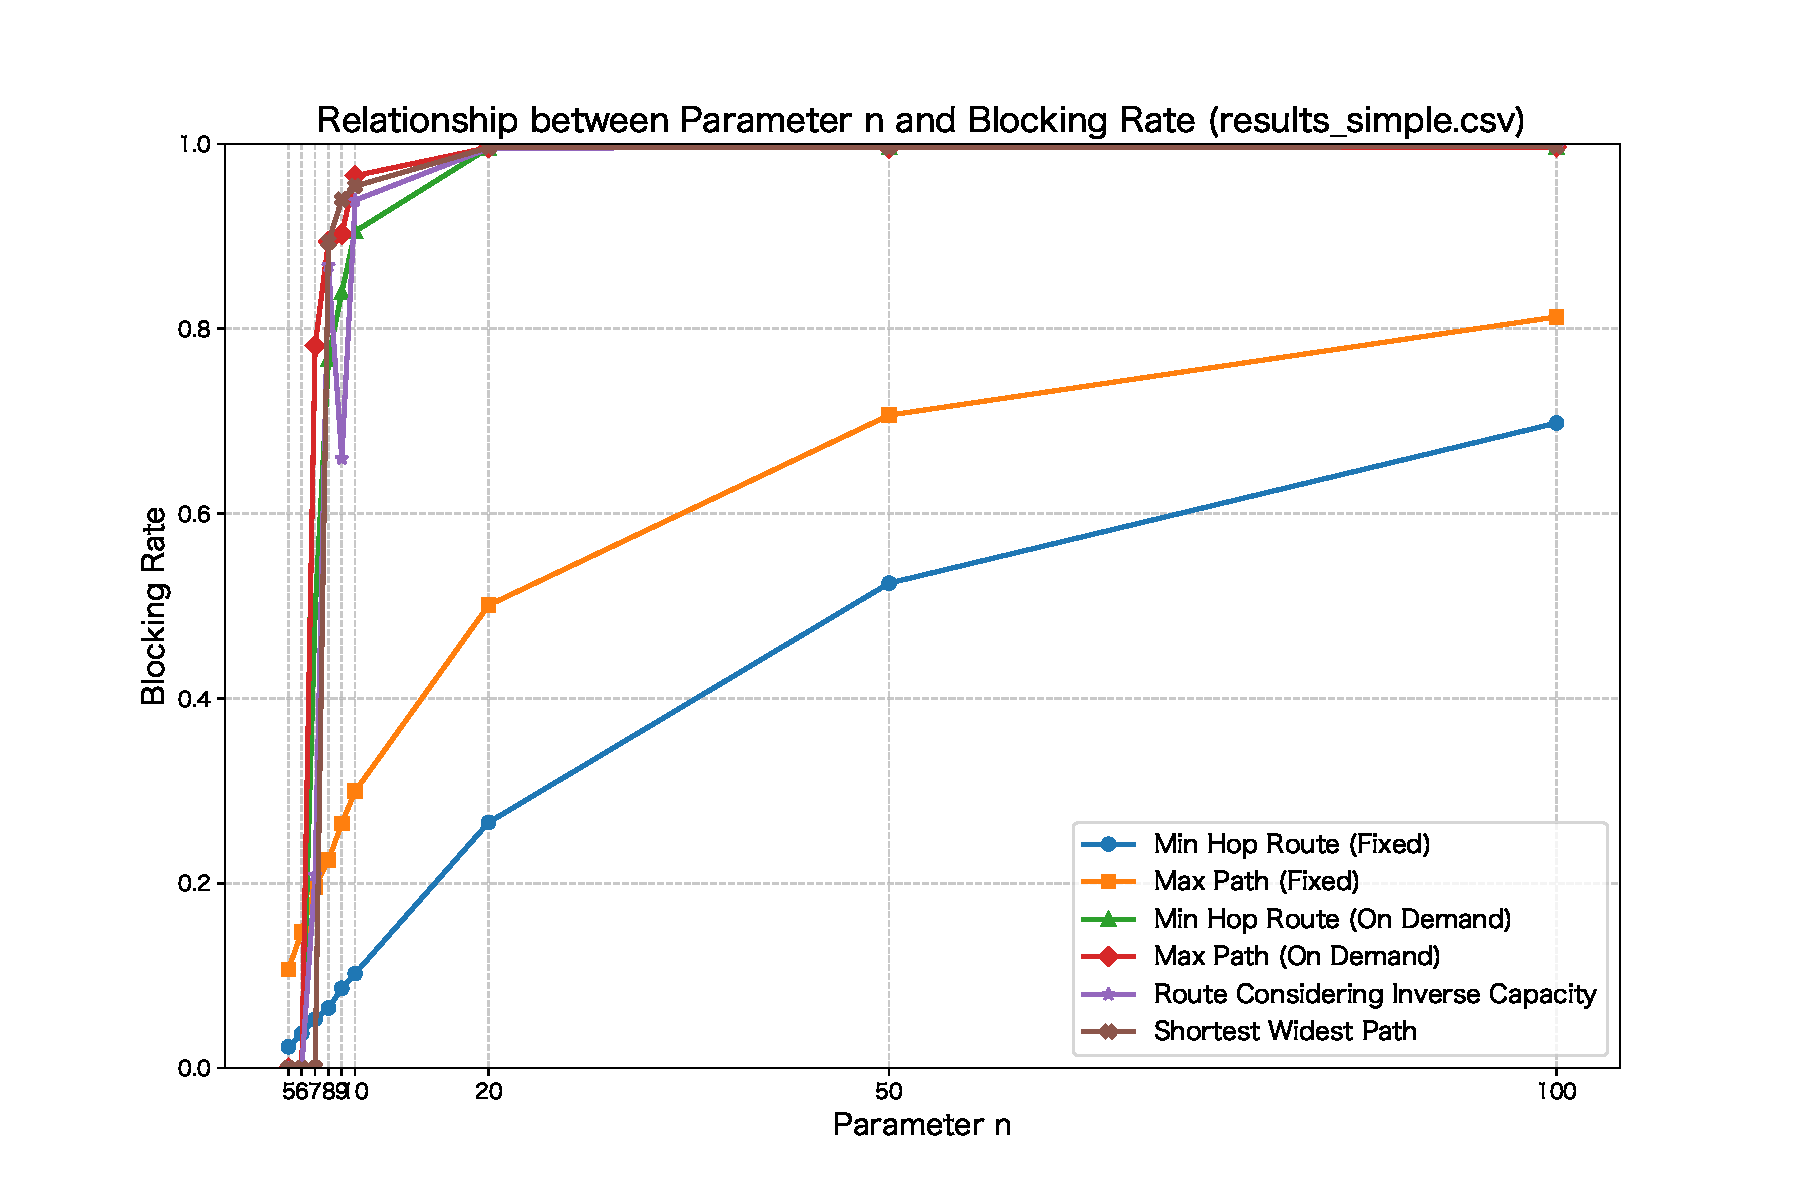
\includegraphics[width=0.9\textwidth,keepaspectratio]{blocking_rate.pdf}
  \caption{パラメータnと呼損率の関係}
  \label{fig:result}
\end{figure}

評価結果から、以下の点が観察された:

\begin{enumerate}
  \item すべての経路選択方法において、パラメータnが大きくなるほど呼損率が増加する傾向が見られた。
  \item n=5の短時間通信の場合、要求時経路選択(最小ホップ、最大路、空き容量の逆数、最短最大路)が非常に低い呼損率を示した。
  \item n=50以上の長時間通信では、固定経路選択(特に最小ホップ固定)が比較的良好な性能を示した。
  \item 最小ホップ経路(固定)は全体的に安定した性能を示し、特に長時間通信においては最も低い呼損率を達成した。
  \item 最大路(固定)は短時間通信では最小ホップ経路より性能が劣るが、帯域を重視する通信には有効である。
\end{enumerate}

\section{考察}

\subsection{経路選択方法の性能比較}
実験結果から、通信時間の長さによって最適な経路選択方法が異なることが分かった。

短時間通信(n=5, 10)の場合、要求時経路選択が非常に低い呼損率を実現した。これは、通信が短時間で終了するため、ネットワークの混雑が生じにくく、その時点での最適な経路を選択することが効果的だからと考えられる。特に、空き容量の逆数を考慮した経路と最短最大路は、n=5において呼損率がほぼゼロに近い値を示しており、短時間通信に対して非常に効果的であることが確認された。

一方、長時間通信(n=50, 100)では、固定経路、特に最小ホップ経路(固定)が比較的良好な性能を示した。これは、長時間の通信が増えると、ネットワークの状態が頻繁に変化し、要求時に最適だった経路が時間の経過とともに最適でなくなる可能性があるためと考えられる。固定経路は、ネットワークトポロジに基づいた安定した経路を提供するため、長時間の通信に対してより堅牢な性能を示すと考えられる。

\subsection{新規アルゴリズムの評価}
本実験で新たに実装した「空き容量の逆数を考慮した経路」と「最短最大路」について考察する。

空き容量の逆数を考慮した経路は、短時間通信において非常に効果的であることが示された。空き容量が少ないリンクを避けることで、通信確立の成功率を高めることができた。特にn=5では呼損率が0.0006と、ほぼすべての通信を確立することができた。

最短最大路も同様に短時間通信で良好な性能を示した。最大の帯域幅を確保しつつ最短経路を選択するという2段階のアプローチは、短時間通信において効果的に機能することが確認された。n=5では呼損率が0.0011と極めて低い値を示した。

しかし、両アルゴリズムともn=50, 100のような長時間通信では呼損率が大きく上昇した。これは、通信時間が長くなると、高い帯域幅を要求する経路が長時間占有されるため、後続の通信要求に対応できなくなるためと考えられる。

\subsection{指数分布による評価手法の意義}
従来の等間隔評価に比べ、指数分布による評価手法を導入したことで、より現実的な通信パターンをシミュレーションすることができた。実際のネットワークでは、通信の到着時間や持続時間は一様分布ではなく、より確率的な性質を持つため、指数分布に基づくモデルはより現実に近い評価を可能にしたと考えられる。

この評価手法により、短時間通信と長時間通信が混在する実際のネットワーク環境でのアルゴリズムの性能をより正確に予測することができるようになった。

\section{まとめ}
本実験では、6種類の経路選択アルゴリズムを実装し、指数分布に基づく通信モデルを用いてその性能を評価した。実験結果から、通信時間の長さによって最適な経路選択方法が異なることが明らかになった。

短時間通信では要求時経路選択(特に空き容量の逆数を考慮した経路と最短最大路)が効果的である一方、長時間通信では固定経路選択(特に最小ホップ経路)が比較的安定した性能を示すことが分かった。

実際のネットワークでは、短時間通信と長時間通信が混在するため、通信の特性に応じて適切な経路選択アルゴリズムを選択することが重要である。また、ネットワークの負荷状況や要求されるサービス品質(QoS)に応じて、経路選択の方針を適応的に変更することも効果的であると考えられる。

今後の課題としては、より大規模なネットワークでの評価や、実際のトラフィックパターンに基づいたシミュレーション、複数の経路選択アルゴリズムを組み合わせたハイブリッドアプローチの検討などが挙げられる。

\section{参考文献}
\begin{enumerate}
  \item 情報通信工学専門実験A 実験テキスト
\end{enumerate}

\appendix
\section{プログラムリスト}
以下に、実装したJavaプログラムのリストを示す。

\lstinputlisting[language=Java, caption=dijkstra.java]{dijkstra.java}

\end{document} 